\documentclass[oneside,a4paper,english,links]{amca}
%
\usepackage{graphicx}
\usepackage{amsmath,amsfonts}

\title{REAL TIME DIRECT VOLUME RENDERING OF BREAD CRUMBS}

\author[a]{Rodrigo Baravalle}
\author[b]{Leonardo Scandolo}
\author[c]{Claudio Delrieux}
\author[d]{Cristian G. Bauza}
\author[a]{Juan C. G\'omez}
%
\affil[a]{Laboratory for System Dynamics and Signal Processing, FCEIA, Rosario National University, CIFASIS-CONICET,
  Ocampo y Esmeralda, S2000EZP~Rosario, Argentina,
  baravalle@cifasis-conicet.gov.ar, \url{http://www.cifasis-conicet.gov.ar/grupo4.html}}
%
\affil[b]{Computer Science Department, FCEIA, Rosario National University,
  Pellegrini 250, 2000~Rosario, Argentina,
  leonardo@fceia.unr.edu.ar, \url{http://web.fceia.unr.edu.ar/es/institucional/escuelas/118-departamento-ciencias-de-la-computacion-ecen.html}}

\affil[c]{Department of Electrical Engineering and Computers, Universidad Nacional del Sur - IIIE-CONICET,
  Col\'on 80, 8000FTN~Bah\'ia Blanca, Argentina,
  cad@uns.edu.ar, \url{http://www.ingelec.uns.edu.ar/}}

\affil[d]{Research Institute PLADEMA- Faculty of Exact Sciences - Universidad Nacional del Centro,
  Paraje Arroyo Seco, (B7001BBO) Tandil, Buenos Aires, Argentina
  crgarcia@exa.unicen.edu.ar, \url{http://www.exa.unicen.edu.ar/es/d_investigacion/inst_pladema/index.html}}


%% NOTE: IF ALL AUTHORS BELONG TO THE SAME AFFILIATION
%% USE THE `\voidaffil' MACRO FOR THE AFFILIATION CODE.
%% Example:
%% \author[\voidaffil]{First A. Author}
%% \author[\voidaffil]{Second B. Author}
%% \author[\voidaffil]{Third C. Author}
%% \author[\voidaffil]{Fourth D. Author}
%% %
%% \affil[\voidaffil]{Grupo de Mec\'anica Computacional,
%% Universidad Nacional de Villa Carolina,
%% Los Alerces 3492, 4200 Villa Carolina, Argentina,
%% gmc@uncarolina.edu.ar, http://www.uncarolina.edu.ar/gmc}

\begin{document}
\vspace{3cm}

\maketitle

%% To set PDF METADATA: uncomment and replace fields in
%% UPPERCASE with appropriate values. 
%% 
%% \hypersetup{
%%   pdfauthor={AUTHORS},
%%   pdfkeywords={KEYWORDS},
%%   pdftitle={TITLE}
%% }
%%
%% For instance
%% \hypersetup{
%%   pdfauthor={Sponge B. and Star P.},
%%   pdfkeywords={multiphase flow, air-liquid mixtures},
%%   pdftitle={A new model for multi-phase flow}
%% }
%%
%% NOTE: To set the metadata is recommended but not absolutely
%% neccesary. 
%% This was done before with the \pdfinfo command,
%% but according to this post:
%% http://de.nntp2http.com/comp/text/tex/2008/12/5358fd061de9703a781885a5dcf98364.html
%% if `hyperref' is used, then you must use \hypersetup{} not \pdfinfo{}

\begin{keywords}
  Direct Volume Rendering, Bread Crumb, Real Time.
\end{keywords}

\begin{abstract}
  Photo-realistic modelling and rendering of materials with complex internal structure poses a hard challenge in the Computer Graphics community. In particular, bread crumbs consist of a complex translucent material with a porous structure that presents different details at different scales. In realistic bread crumb rendering there are several light phenomena involved such as subsurface scattering, self-shadowing, self-occlusion, reflectance, and absorption. Current approaches to recreating these phenomena using a realistic approximation of the rendering equation, i.e., accounting for global illumination as in ray and path tracing, are computationally expensive and generally require a detailed mesh of the bread crumb.

  State of the art techniques for bread crumb rendering set up a complex capture procedure, in which the light reflecting off the material is sampled at different angles. That information is used to reconstruct a material model. While this solution accounts for several desired properties of this material, it presents several drawbacks which makes difficult its practical applications: high computational costs, the requirement of complex capture procedures, and poor image variability.

  In this work, we propose the study and implementation of a GPU based direct volume rendering on a scalar field representing the internal structure of a bread crumb without requiring any intermediate steps. The images obtained show promising results at interactive and real time frame rates. The crumb is represented as a 3D scalar field, which is computed in two steps. The first uses a particle-system based generation procedure, and the second uses dynamic systems to evolve the particles mimicking the bread making process.
\end{abstract}

\section{INTRODUCTION}

The appearance of bread crumbs and other baked materials, such as
pizzas and cookies, has been considered challenging to render due to
the complex interaction of light outside and inside the
material. Computational costs (memory storage and cpu time) of these
physical simulations made its rendering impractical in areas in which
interaction with the final user is critical. The exponential growth in
computing power, based on the massively parallel design of modern
graphics cards \citep{Yeo09,Harris06}, has made it possible to
simulate some light phenomena at acceptable computational rates, but
the field is still a subject of research \citep{Voglsam2013}.

The geometry of these materials represents an additional challenge. These porous structures are the
result of complex mechanisms which involve physical deformations and
chemical reactions. In bread making, two different
processes are involved: proofing and baking. Proofing involves
chemical reactions between the living yeast and the dough. The yeast
produces $CO_{2}$ which in turn makes bubbles in dough
\citep{Shah1998}. In the baking process \citep{Mondal2008},
temperature changes these shapes in several ways \citep{Scanlon2001},
giving bread its final internal structure. A few attempts to
synthesise a model of the resulting geometrical structure have been
made \citep{VanDyck2014,Cho2007}, but the structure obtained is the
result of an artistic design, and, in the case of x-ray tomography,
the variability of the structure is limited to the amount of captures
made. In this work we propose to employ dynamical systems
\citep{Strogatz2001} in order to evolve particle systems
\citep{Reeves83} that we have previously designed
\citep{Baravalle2011}, trying to mimic the bread making process
(proofing and baking). Many complex processes, such as weather and
fluids, are governed by differential equations which describe their
dynamics and appearance. This idea is employed in this paper in order
to describe the bubble growth process in bread. This process produces a
structure which is perceived as if bubbles were growing inside a fluid,
similar to patterns found in bread crumbs. Other approaches compute
texel values using algebraic functions so they do not require to
store a 3D texture in memory \citep{Perlin1989}, but in our case this
method is not adequate since the bubble distribution is difficult to
capture with a statistical approach.

The mechanism for rendering the internal constitution of these materials largely depends
on the data structure chosen for its representation. When triangular
meshes are used, they should be computed from voxel data, using
techniques such as marching cubes \citep{Lorensen1987}. Nevertheless
such process could be a non-trivial task due to the porous bread structure, and it
could potentially hold a large amount of information in memory. Surface representations
of this material are not adequate since it presents visible structures on it.
Bread is classified as a quasi homogeneous material \citep{Tong2005}, due to the presence
of mesostructures (bubbles) on its visible surface. In other words, typical solutions such as
Bidirectional Reflectance Distribution Functions (BRDF)
\citep{Kurt2009} and Bidirectional Surface Scattering Reflectance
Distribution Functions (BSSRDF) \citep{Donner2009} are not completely
adequate since mesostructures cannot be addressed with these
methods. These limitations are solved by a material model \citep{Tong2005}. Although this method shows good results, the associated drawbacks (complex capture procedure
involved, computational costs, poor image and structure variability),
made its widespread application very difficult.

In this paper we propose to apply Direct Volume Rendering (DVR)
\citep{Levoy1988,Kruger2003, Kratz2006} on a scalar field to render
the bread crumb structure. DVR applies ray marching through a volume
accumulating different properties for each pixel. The method does not
use intermediate structures, which simplifies the modelling
process. In addition, the shape of the bread crumb can be defined in
real time on the GPU, making it possible to perform arbitrary cuts,
slices and deformations of the 3D structure in real time. Also, the
bread crust can be easily defined along with its own properties like
colour and translucency using transfer functions. Satisfactory results
are obtained at real time rates.

This paper is organised as follows. In section 2 the theory of
particle systems, dynamical systems and DVR is introduced. In section
3 the results obtained in the 3D structure generation and rendering
are shown and discussed. In section 4 the conclusions are summarised,
as well as possible future works.

\section{MATERIALS AND METHODS}

\subsection{Particle systems}

Early approaches in computer graphics tried to represent nature by employing Euclidean geometry. In other words, combining points, lines, surfaces, spheres, cylinders, cubes, and other simple primitives. Nevertheless, it is difficult to capture details of natural structures with this approach. The shape observed in mountains, coastlines,  and almost every natural object presents irregularities which are difficult or impossible to represent using these primitives. Other approaches such as fractal geometry \citep{Mandelbrot83} emerged and claimed to describe natural phenomena more adequately. With this new perspective, previous phenomena could be better modelled and rendered. 

Several techniques for representing non-Euclidean
objects simultaneously appeared. Particle systems \citep{Reeves83} were designed for
dealing with phenomena which have no well defined surface, like water,
smoke, and fire. Particle systems are composed of entities called {\em
  particles} which evolve its properties over time. As an example, for
rendering fireworks a particle system in which each
particle begins its trajectory in a common space position is defined, and after
each time step its position is modified following a parabola. Different
particles follow slightly different parabolas. An image is obtained at
each step and an animation can be seen. For obtaining other effects as fire, properties as colour, size and direction are modified
depending on time. Particles can also affect each other.

In a previous work \citep{Baravalle2011}, particle systems were employed for texture synthesis. Each particle had an initial random position in the image, and evolves trying to avoid other particles. Adequate results were obtained for wood and painting textures. The growing functions used were mainly random, vertical, horizontal and diagonal. In this work, an extension into space is proposed, and also the use of a system of differential equations to control the growth of the self-avoiding particles for mimicking the bread making process, obtaining a 3D texture for representing this material. 

\subsubsection{Algorithm for particle systems}
This algorithm's purpose is to produce a geometry which will be rendered in a later step. Therefore, instead of delivering the colour of a particular space position it will generate a scalar field composed of $0$s and $1$s ($0$ if the position contains air, $1$ if the position contains mass). This representation is adequate for DVR.

The system consists of a set of particles $P$, 

\begin{equation}
  P = \{p_{1}, ... , p_{n}\}, n  \in \mathbb{N},
\end{equation}

\noindent a lattice $L_{N\times N \times N}, N \in \mathbb{N} $ (initially $L_{xyz}=1$) of mass and air as described before (the output of the algorithm), and a lattice $L2_{N\times N \times N}$, (initially $L2_{xyz}=-1$), of positions and particle ownership ($i$ if the lattice element belongs to the contour or interior of the particle $i$).

Each element in $P$ has the following properties:

\begin{equation}
  p_{i} = \{O_{i}, C_{i}\}, 1 \le i \le n,
\end{equation}

\noindent where:

$O_{i} = \{o_{1}, ... , o_{n_{i}}\}$: (Occupied) vector (set) of occupied positions by the particle in $L$.

$C_{i} = \{c_{1}, ... , c_{m_{i}}\}$: (Contour) vector (set) of positions representing the {\em contour} of the particle in $L$. The vector $O$ represents the positions which will be affected by the particle, and the contour $C$ is created to ensure avoidance with other particles.

The algorithm works as follows. Each particle evolves trying to extend
its occupied positions ($O$) by marking positions in $C$. When a
position is marked, it is deleted from $C$ and added to its $O$
vector. The neighbourhood of that position, {\em i.e.}, the lattice
positions surrounding it, are added to the contour vector $C$. The
lattices are also updated: $L$ is set to $0$ in $O$ (the air
bubble is now bigger), and $i$ is set in $L2$ to the neighbourhood
positions. In practice, the neighbourhood size is a parameter, so
different distances between particles can be defined.

When $t = 0$, a set of initial particles take random positions in the lattice. The position chosen is the first lattice position which will belong to $O$ and the surrounding positions are added to $C$. Also, the lattices are updated accordingly. Then, for each $t$, each particle chooses a position on its contour, and the presence of other particles is checked on it. This is done in the lattice $L2$. If the position lies in the contour of any other particle ($L2_{position} <> i$ and $L2_{position} > -1$), the position is discarded and the process continues, selecting another contour position. If that position is not in the contour of another particle ($L2_{position} = i$ or $L2_{position} = -1$), the particle adds the position to its $O$ and updates its contour $C$ (and again the lattices $L$ and $L2$). If the contour vector is empty, the particle {\em dies}, since it cannot grow anymore in the simulation.

Termination of the algorithm is possible at any $t$. It could also be set to stop at a particular event, for instance, when the $L2$ lattice is full ($L2_{xyz} <> -1$ in any lattice position), since no progress can be made.

Different structures are produced varying the contour size (see Fig.~\ref{fg:fig1}). The image shows 2D output examples (for better understanding) of random growing particles. The white region among particles (mass) is determined by the contour size, in other words, the {\em width} of the white area. Resulting images seem to form voronoi-like patterns.


\begin{figure*}[htb!]
  \centerline{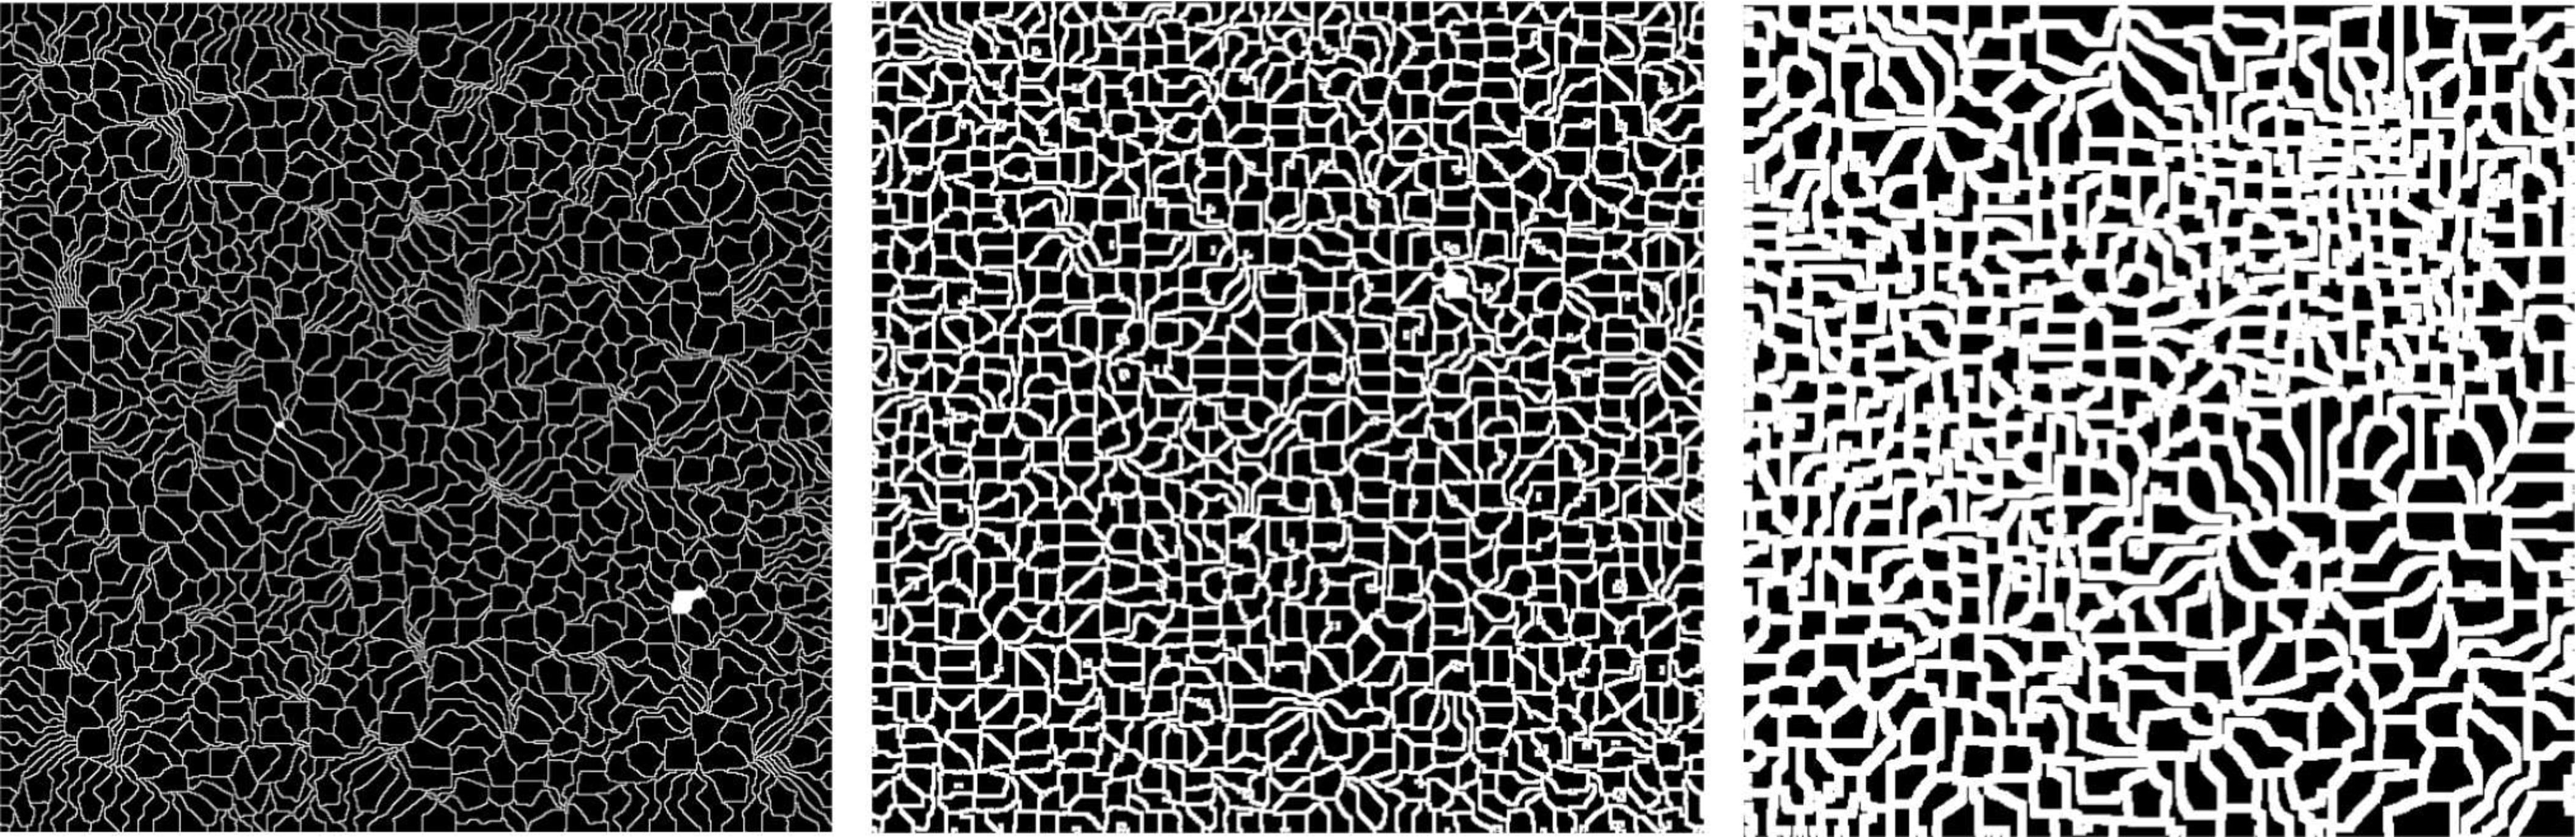
\includegraphics[scale=0.22]{fig1.pdf}}
  \caption{Different sizes of the contour parameter. Left: contour = 1, middle: contour = 2, right: contour = 4.}
  \label{fg:fig1}
\end{figure*}

The $L$ lattice is the output of the algorithm, and it represents the
structure which will be rendered. The
next section establishes the system employed to evolve the particles
over time.

\subsection{Dynamical systems}

The subject known as Dynamics deals with {\em change}
\citep{Strogatz2001}. The study of Dynamics began in previous
centuries with Isaac Newton's works. Among his contributions,
Differential Equations can be found. These help manage the
difficulty (or impossibility) of finding analytical equations for
these dynamical processes. A model describing the problem is
first defined from which differential equations are derived. The
evolution of the system is simulated and approximate solutions are
derived for each step of the simulation. Dynamical systems are
concerned about processes that evolve in time, such as economics, heat
transfer, and fluids. With the development of computers in the last
century, the field has been able to obtain insight into areas which
were unexplored before, since the calculations were too difficult to
be performed by humans, for instance, Fractals \citep{Mandelbrot83}
and Chaos.

Numerical approximations are used to solve dynamical systems. Its computational costs change depending on the complexity of the problem and the number of equations involved. We propose to employ a sub field of differential equations, Ordinary Differential Equations (ODE), for the purposes of this work. In ODEs, time is treated as the only variable, and the equations show the relationship between the derivatives of the variable and the variable itself. 

Generally speaking, ODEs can be represented using the following set of equations:
\begin{equation} \label{eq:simple}  
  \begin{aligned}
    \dot{x_{1}} = f_{1}(x_{1},\ldots,x_{n}),\\
    \ldots\\
    \dot{x_{n}} = f_{n}(x_{1},\ldots,x_{n}),
  \end{aligned}
\end{equation}

\noindent where $\dot{x_{i}}$ represents the derivative of $x_{i}$ with respect
to the variable $t$. The variables $x_{i}$ and the functions $f_{i}$
are defined for each problem. In this work, each variable represents a
Cartesian coordinate in space, {\em i.e.,} $x_{1}$ is $x$, $x_{2}$ is
$y$ and $x_{3}$ is $z$ and the set of $f_{i}$ will be defined in order
to capture the bread crumb structure. The next section shows how these
systems can describe the evolution of a particle evolution.

\subsection{Evolution of particle systems using dynamical systems trajectories}

Human perception can detect patterns in bread crumb structure. Key
observations can be made in real images of bread crumbs (see
Fig.~\ref{fg:fig2}). First, if close to the crust, bubble shape tends
to follow the crust shape. This is not casual, since temperature in
baking affects the bubbles' shape \citep{Scanlon2001}, stretching
them following its walls. Another observation is that the entire
structure has a fluid appearance. Indeed, this is the case in
early stages of the baking process. At some point, the viscosity
of the dough decreases and the bubbles cannot continue growing and
coalescing.

\begin{figure*}[htb!]
  \centerline{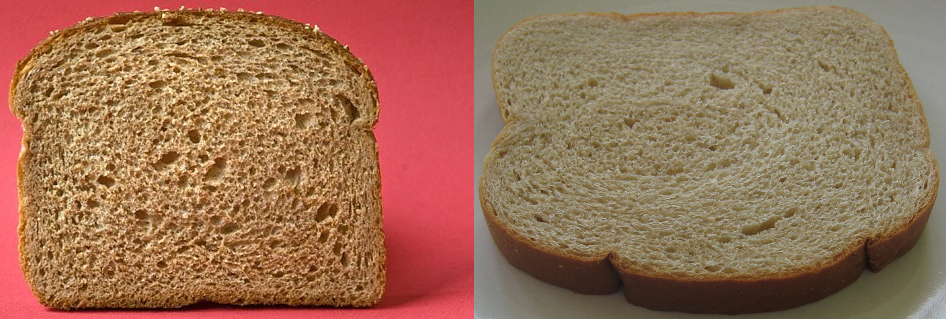
\includegraphics[scale=0.45]{fig2}}
  \caption{Images of real bread slices}
  \label{fg:fig2}
\end{figure*}

Dynamical systems produce natural shapes (see
Fig.~\ref{fg:fig3}). Circles and spirals can be seen if trajectories
are defined over their domain. Three different set of equations
describe the dynamics in each of the images. For instance, the left
one is produced by the following set of equations:

\begin{equation} \label{eq:simple}  
  \begin{aligned}
    \dot{x} &= x^{2}-y^{2}+1,\\
    \dot{y} &= 2xy+1.
  \end{aligned}
\end{equation}


\begin{figure*}[htb!]
  \centerline{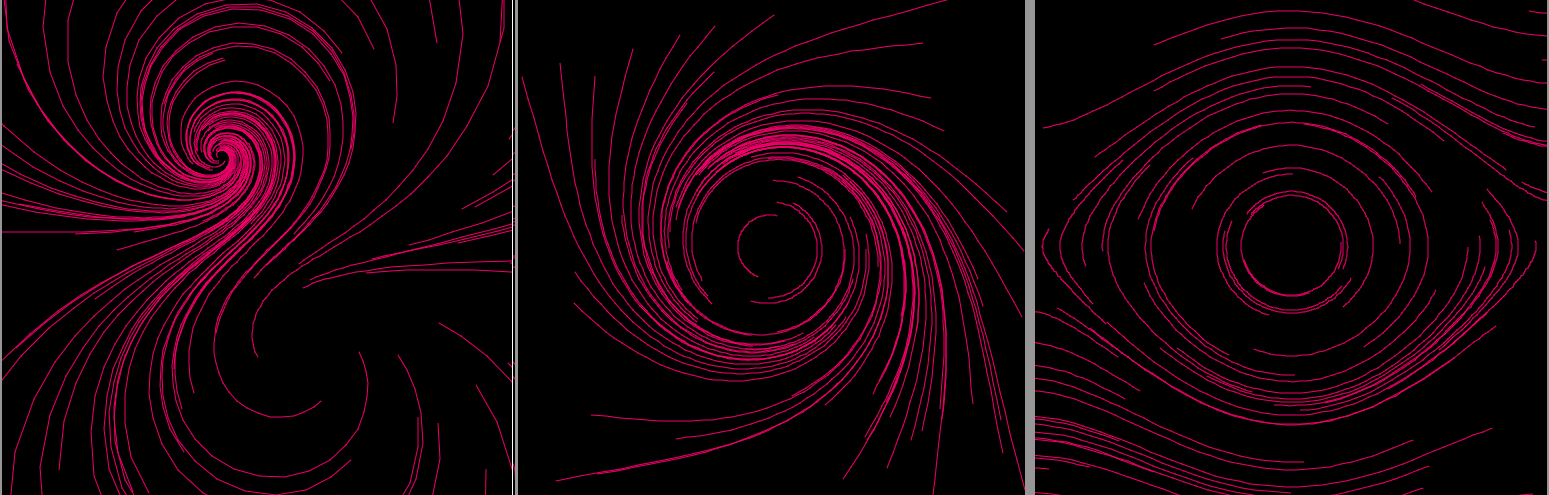
\includegraphics[scale=0.28]{fig3}}
  \caption{Dynamical systems in the plane.}
  \label{fg:fig3}
\end{figure*}


Random positions are chosen in the examples, and then the system is solved at each time step using a fourth order Runge-Kutta solver to determine the new trajectory direction. In the left image, the trajectories are {\em attracted} by a position which lies in the left-upper quadrant. Trajectories could also be attracted to a set of points instead of a single one. In the right image, trajectories follow circles and other shapes without having a point attractor (the entire shape is an attractor).

Patterns can be produced by particles following trajectories in the plane or space. In order for a particle to follow a trajectory, the dynamical system is solved at the current position of the particle, and the contour position which best approximates that solution is chosen for growing. In other words, the dynamical system defines a vector field that could be used by the particles.

When the particles' growing direction is set to follow this vector field, bubbles are globally deformed in a similar shape as the
trajectories of the dynamical system (see Fig.~\ref{fg:fig4}). In the
images, from left to right, the trajectories' {\em randomness} is decremented. The right image was produced with randomness set to $0.1$, meaning
that the bubbles are forced to follow the dynamical system
trajectories with a probability of 0.9. This probability is defined as
$1-randomness$, with $0 \leq randomness \leq 1$. The dynamical system
used is the same as the right image shown in Fig.~\ref{fg:fig3}.  The
patterns are adequate for use not only in bread images, but also
cakes, and other baked foods, varying the randomness
parameter. Different useful structures could be defined by different set of equations and different parameters for the
particle systems (lifetime of particles, randomness).


\begin{figure*}[htb!]
  \centerline{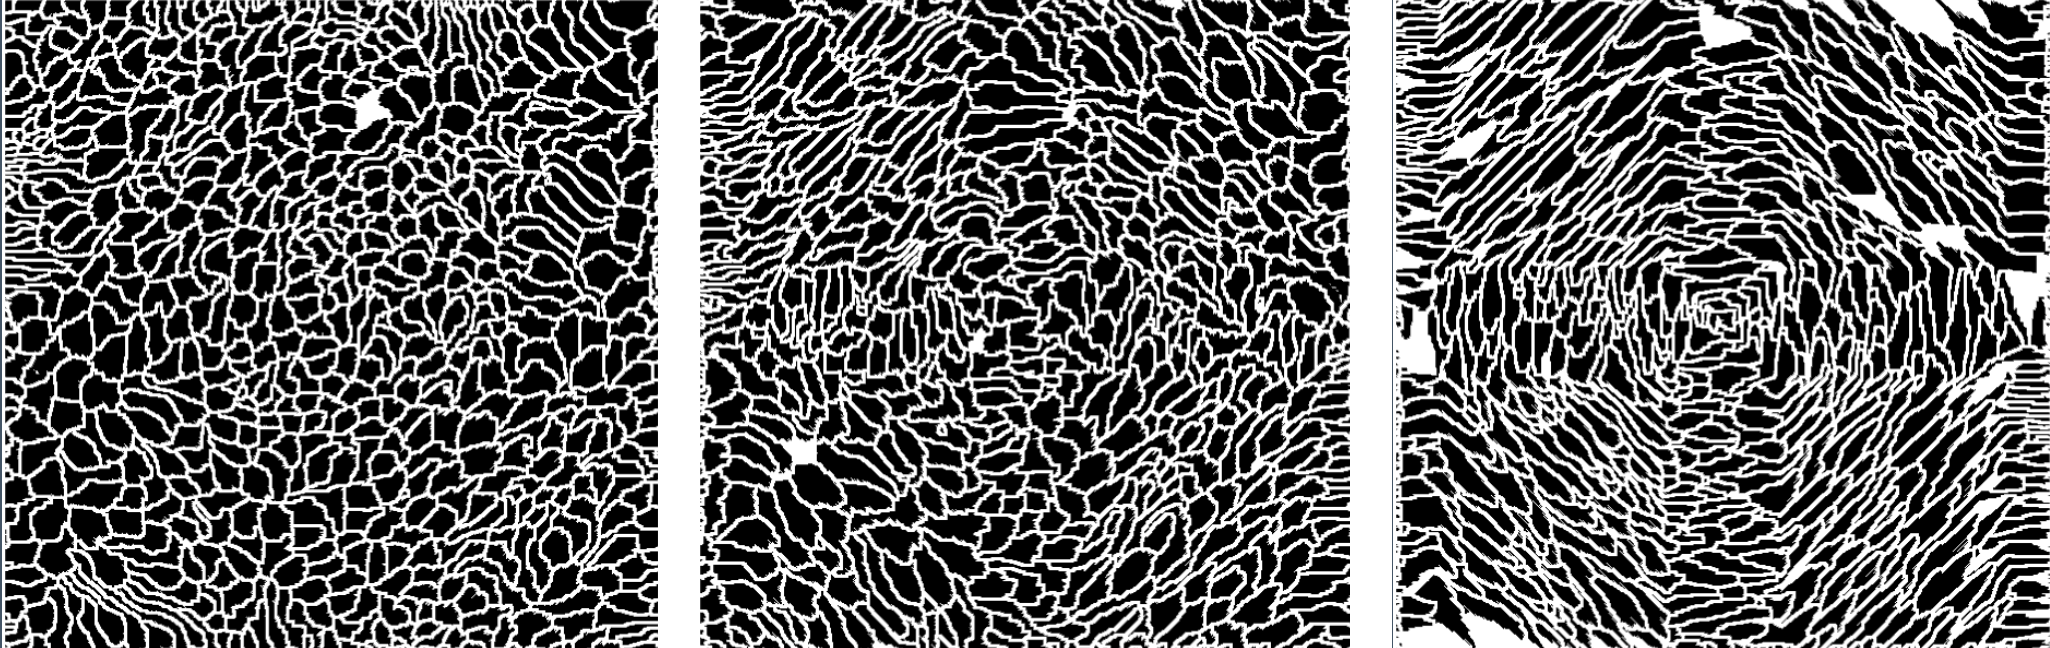
\includegraphics[scale=0.21]{fig4}}
  \caption{Dynamical systems affecting particle systems. Effect of the randomness parameter. From left to right, randomness: 0.3,0.2,0.1 respectively. }
  \label{fg:fig4}
\end{figure*}

The next section shows how these evolved particles can be rendered.

\subsection{Algoritmo de renderizado}

En esta sección explicaremos la teoría de la técnica de DVR y se
presentarán algunos aspectos de la implementación usada en este
trabajo.

\subsubsection{Direct volume rendering}

La técnica de DVR tiene como objetivo crear una representación
bidimensional de un volumen definido por una función de densidad
tridimensional. Para ello, se emiten rayos desde el punto de vista de
una camara en una escena virtual y se utiliza la función de densidad
para calcular la cantidad de luz que la cámara recibe en la dirección
del rayo. Para esto se evalúa la función de densidad en el camino del
rayo y se usan los valores adquiridos para aproximar el efecto de
varios fenómenos lumínicos, como pueden ser la extinción,
transmitancia, o dispersión lumínica, entro otros. La información
obtenida de procesar todos los rayos se usa para definir el color de
los pixeles en la imagen final.

La radiancia es la cantidad de luz que pasa, o es emitida, desde un
punto y atraviesa un determinado ángulo sólido. En el contexto de DVR,
el medio que los rayos atraviesan, y que es definido por una función
de densidad, es considerado como emisivo. Por lo tanto, cuando se
busca calcular la cantidad de luz recibida en la dirección de un rayo,
lo que se hace es aproximar la radiancia recibida de un punto distante
siguiendo la dirección del rayo. El valor de la radiancia es
aproximado como la suma de una radiancia de fonto y la radiancia
emitida por el medio por el cuál se mueve el rayo \citep{Kratz2006} :

\begin{equation} \label{eq:general_radiance}  
  L(p_n) = L_b + \int_{p_0}^{p_n} \frac{\partial L(t)}{\partial p} \, dt,
\end{equation}

\noindent donde $L_b$ es la radiancia de fondo, $p_0$ y $p_n$ son los
puntos inspeccionados en la dirección del rayo más cercano y más
lejano respectivamente, $L(t)$ es la radiancia evaluada en el punto
$t$, y $\partial p$ es la distancia entre puntos evaluados. En el
momento de calcular $L(p_n)$, la integral es aproximada por una suma.

La extinción es la pérdida de fotones en un haz de luz debido a la
absorción en el medio que atravieza y la dispersión hacia otras
direcciones. Algunos de los fotones colisionarán con particulas del
medio y serán absorvidas y transformadas en otras formas de energía,
mayormente calor. Otras rebotarán y pasarán a moverse en otras
direcciones. Estos fenómeno son aproximados usando un coeficiente de
absorción para el medio, $k_a$ y un coeficiente de dispersión
$k_s$. Si el efecto de dispersión es ignorado, la fórmula que define
la cantidad de radiancia absorbida en el largo de un segmento de rayo
es: 

\begin{equation} \label{eq:radiance_absorption}  
    L_b \ \displaystyle e^{-\int_{p_0}^{p_n} k_a(t) \, dt}.
\end{equation}

El valor $\int_{p_i}^{p_j} k_a(t) \, dt$ es llamado coeficiente de
absorción y será referenciado como $\tau_{(p_i, p_j)}$.

La transmitancia es un concepto complementario a la extinción y
describe la cantidad de luz que pasa por un medio en una dirección
determinada. El valor de transmitancia entre dos puntos $p_i$ y $p_j$
es:

\begin{equation} \label{eq:general_radiance}  
  T(p_i,p_j) = e^{-\tau_{(p_i, p_j)}}.
\end{equation}

Si la emisión de luz se asume como un término constante ($\rho$) para
todos los puntos del medio, la fórmula inicial de radiancia queda:

\begin{equation} \label{eq:ray_radiance}  
  L(p_n) = L_b \ e^{-\tau(p_0, p_n)} + \int_{p_0}^{p_n} \rho \ e^{-\tau(t,p_n)} \, dt.
\end{equation}

Esto significa que la radiancia entre los puntos $p_0$ y
$p_n$ se puede calcular como la radiancia de fondo restante luego de
la atenuación del medio sumada a emisión, también atenuada, en todos
los puntos del medio que atraviesa el rayo.

La técnica de DVR define un volúmen donde una función de densidad se
evalúa en intervalos regulares y utiliza esa información para
aproximar la transmitancia en esos puntos y de esa manera aproximar la
cantidad de luz que llega a la cámara. La suma integral descrita
anteriormente se reemplaza por una suma discreta de los puntos
evaluados de un rayo donde este intersecta al volumen que interesa
representar. 

Otros efectos lumínicos pueden ser aproximados. Esto aumenta la
fidelidad de la imagen final pero también aumenta el costo de cómputo
de la técnica. Algunos de estos efectos son el cálculo de fase, de
luz entrante por dispersión o luz extinguida por dispersión, entre
otros. Dado que el objetivo de este trabajo es lograr un renderizado
en tiempo real, el algoritmo implementado usa como base el modelo de
cálculo de radiancia simplificado que toma en cuenta sólo la
transmitancia del medio.

\subsubsection{Implementación}

\paragraph{Sinopsis}

Un programa de prueba \footnote{disponible en
  \emph{\url{https://www.github.com/rbaravalle/Pysys}}} fue creado
para evaluar el sistema de partículas que describe la estructira del
pan. Este programa usa el sistema de partículas para generar una
textura volumétrica que se interpreta como una función de
densidad. Esta textura se usa como entrada para un renderizador basado
en DVR que genera imágenes del pan representado por el sistema de
partículas original. Este programa demuestra que el método de
renderizado propesto es compatible con los motores gráficos basados en
técnicas de renderización en tiempo real en GPU. Se obtienen imágenes
de un material realístico así como efectos de sombras suaves dentro
del volúmen. Esto significa que las técnicas usadas para renderizar
esto materiales pueden ser integradas en cualquier motor de
renderizado que soporte shaders.

\paragraph{Detalles}

La malla que utiliza el modelo es un cubo que contiene el volúmen
definido por el sistema de partículas original. El código del shader
de vértices es muy simple, proveyendo sólamente información geométrica
al shader de fragmentos. Este último es donde se encuentra la mayor
parte de los cálculos a realizar.

Dentro del shader de fragmentos lo primero que se hace es calcular la
geometría de un rayo cuyo origen es la cámara de la escena y cuya
dirección lo lleva hacia el fragmento siendo calculado. Este rayo es
recorrido en intervalos regulares, evaluando la textura volumétrica
para obtener la densidad del pan en esos puntos. Este valor se utiliza
para calcular la transmitancia acumulada desde la cámara hasta el
punto evaluado. Una vez que la transmitancia es menor que un valor
preestablecido o el rayo sale del cubo que define el volúmen, el
cómputo termina.

En cada punto evaluado también se evalúa la transmitancia dentro del
volúmen desde el punto hacia la fuente de luz en la escena. Esto se
hace emitiendo un rayo desde el punto evaluado con dirección a la luz
y nuevamente evaluando la densidad en varios puntos del rayo. Con esta
nueva información se aproxima la cantidad de luz que llega
directamente al punto evaluado, y permite representar sombras dentro
del volúmen.

La información de transmitancia de los puntos evaluados del rayo
principal y desde estos puntos hacia la transmitancia hacia la luz son
utilizados para calcular el color final del fragmento. A partir de
esta información y tomando diferentes consideraciones artísticas
pueden lograrse representaciones realisticas de diferentes
materiales. En el caso de las imágenes de muestra presentadas en este
trabajo el color del fragmento será más oscuro para areas del volúmen
que se consideran dentro de la corteza del pan y será de un color
amarillo claro para la miga. También se usa un componente especular
tenue. La información de transmitancia entre los puntos evaluados y la
luz ayuda a proveer detalles de la estructura del pan.

El programa de prueba creado permite modificar parámetros tales como
el coeficiente de transmitancia del pan, el límite de transmitancia,
el color asignado a la miga y la fuerza de los reflejos especulares,
entre otros. Esta capacidad permite crear imágenes que semejan otros
materiales porosos, como por ejemplo esponjas. En la siguiente sección
se presentan y se evalúan los resultados obtenidos.

\section{Resultados}

En esta sección se detallan las imagenes y los tiempos de
cómputos obtenidos. 

\subsection{Resultados del renderizado}

Las imágenes que fueron obtenidas a partir del método descrito en la
sección anterior fueron renderizadas en una computadora con una placa
gráfica nVidia GTX 480 ($480$ cores), la cual es normalmente de uso
hogareño. La CPU fue una Intel(R) Core(TM) i5-2300 CPU (cuatro
procesadores). La resolución de las imágenes es de $1440\times990$
pixels. 
Se obtuvieron diferentes imágenes que semejan materiales
horneados. Diferentes tipos de pan pueden ser representados a partir
de cambiar los parámetros de transmitancia y colores utilizados (ver
Fig.~\ref{fg:fig5}). En la imagen del medio los patrones producidos
por los sistemas de partículas descritos en las secciones previas son
claramente visibles. En ese caso, el tiempo de vida de las particulas
es diferente para cada una y de esa manera se obtienen burbujas de
diferentes tamaños.

\subsection{Corteza, fetas y cortes}

Se define una función para determinar si un punto del volúmen es parte
de la corteza o parte de la miga del pan. Por ejemplo, un pan de forma
cilindrica puede determinar que un punto es parte de la corteza si el
punto está a más de cierta distancia del eje del cilindro, y miga en
otro caso. Otra función define si un punto debería considerarse vacío,
más allá del valor de la textura volumétrica en ese punto. Esto
permite definir fetas de manera simple. Por ejemplo, se pueden crear
fetas definiendo una función que asigna aire en intervalos fijos en un
solo eje. Esto produce prismas de aire en el volúmen, como puede
apreciarse en las imágenes obtenidas (ver Fig.~\ref{fg:fig5},
Fig.~\ref{fg:fig6}). 

%% A function defines whether a point in the volume is part of the crust
%% or part of the crumbs. For instance, a cylindrical bread could define
%% a position as crust if the point has certain distance to the centre of
%% the volume (in $X,Y$ coordinates, for all $Z$) , and crumb when its
%% distance is lower. Another function defines whether a point should be
%% considered empty air. This allows an easy way to define slices in the
%% bread. For example slices could be defined by returning true if the
%% modulus of the z coordinate division in the position vector with
%% certain number is $0$ (the width of the slice).  This produces prisms
%% of air in the volume which resemble slices as can be seen in the
%% images (see Fig.~\ref{fg:fig5}, \ref{fg:fig6}).

La asignación de espacios de aire y de corteza deberían extenderse más
allá de ecuaciones basadas en posiciones para poder ser usadas en un
proceso artístico.

\begin{figure*}[htb!]
  \centerline{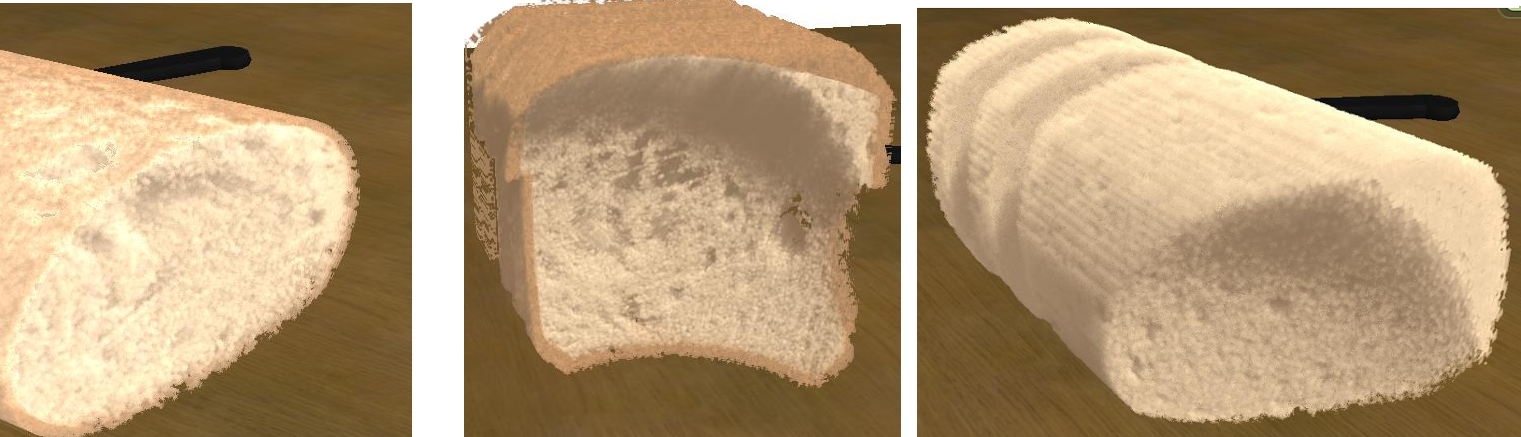
\includegraphics[scale=0.3]{fig5}}
  \caption{Imágenes de diferentes tipos de pan renderizados en tiempo
    real. La imagen de la derecha muestra un pan sin corteza}
  \label{fg:fig5}
\end{figure*}

Pueden obtenerse otros materiales (ver Fig.~\ref{fg:fig6}). Estos son
el resultado de la variación de parámetros técnicos y artísticos del
modelo. En las imágenes de prueba pueden distinguirse un budín (izq.), un
pedazo de torta (medio) y una esponja (der.). En el caso de la esponja
se modificaron los parámetros que definen la función de
densidad. Cuando no hay levadura en el proceso de creación puede
utilizarse una textura volumétrica cuyos valores provienen de una
función aleatoria. La retroiluminación también puede aproximarse con
este modelo (ver Fig.\ref{fg:fig7}). En esa imagen puede apreciarse
una esponja retroiluminada y se puede apreciar la propagación de luz a
través del volúmen que representa.

\begin{figure*}[htb!]
  \centerline{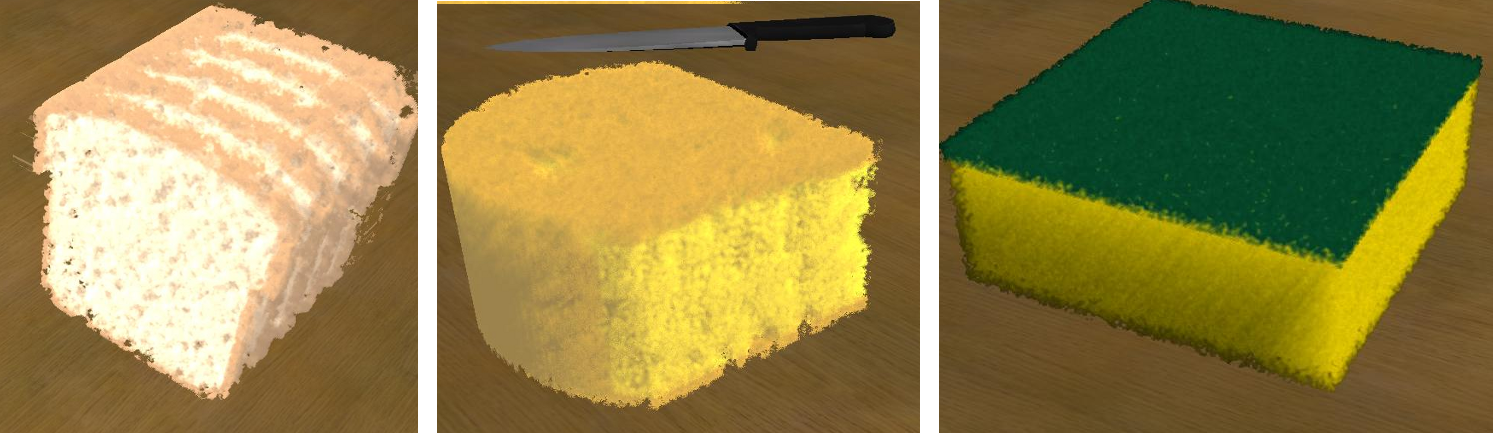
\includegraphics[scale=0.3]{fig6}}
  \caption{Otros materiales renderizados en tiempo real con distintos parámetros. Izq.: budín, medio: torta, der.: esponja. }
  %% \caption{Other materials rendered in real time changing parameters in the model. Left: sliced pudding, middle: slice of cake, right: sponge. }
  \label{fg:fig6}
\end{figure*}



\begin{figure*}[htb!]
  \centerline{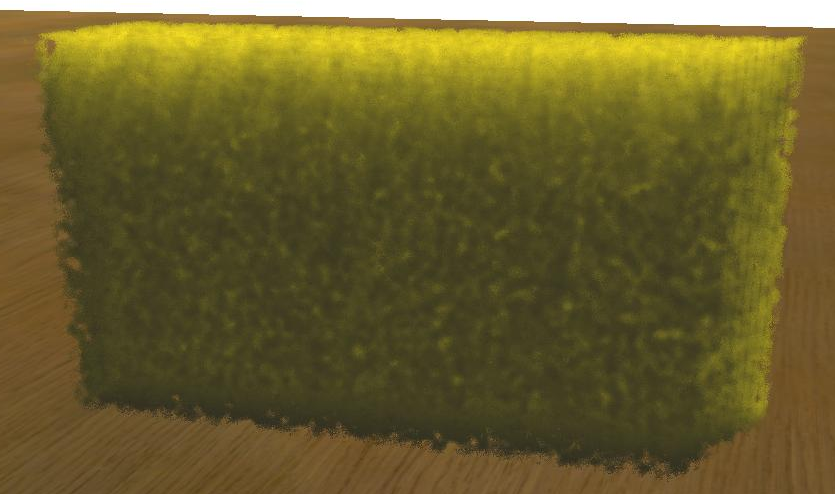
\includegraphics[scale=0.25]{fig7}}
  \caption{Esponja retroiluminada.}
  %% \caption{Sponge showing back illumination in the model. }
  \label{fg:fig7}
\end{figure*}


\subsection{Tiempos de cómputo}

La mayoría de las imágenes fueron obtenidas con tasas de refresco de
tiempo real (más de 30 FPS), como muestra la tabla~\ref{tab:n1}. La
eficiencia del proceso se resiente cuando la transmittancia es muy
baja (el material es casi transparente), dado que se evaluarán más
puntos en los rayos a recorrer antes de llegar al límite de
transmitancia. Otro parámetro importante es la distancia entre puntos
a evaluar. Experimentalmente se encontró que para todos los casos
evaluar $100$ puntos o más da buenos resultados. El proceso escala
automáticamente con el numero de procesadores en una GPU, por lo cual
la tasa de refresco obtenida será mayor en GPUs más rápidas y de más
procesadores.

\begin{table}[htb]
\centering
\begin{tabular}{|c|c|c|c|c|c|c|}
\hline &  Pan 1 & Pan 2 & Pan 3 & Budín & Torta & Esponja \\
\hline
\hline
 FPS promedio  & 32.2 &  75.5 &  45.2 & 28.5 &  54.2 & 29.7\\
\hline
 Puntos de evaluación &  140 &  140 &  140 & 256 &  140 & 256 \\
\hline
 Transmitancia &  15 &  15 &  15 & 15 &  15 & 2.25 \\
\hline
\end{tabular}
\caption{Tiempos de cónputo y parámetros de las imágenes de prueba.}
%% \caption{Computing times and key parameters for the images obtained. }
\label{tab:n1}
\end{table}

\subsection{Conclusiones}

Hasta donde conoce el autor, este es el primer intento de renderizar
pan de manera realistica en tiempo real sin el uso de procesos
intermedios complicados (captura de imágenes, generación de mallas,
post-procesamiento). Ha habido buenos resultados de renderizado de pan
obtenidos con otros métodos (\citep{Cho2007}), pero es dificil
comparar ese trabajo con el presentado en este artículo debido a que
ni los detalles de la técnica utilizada ni los tiempos de cálculo han
sido publicados.

Dentro del volúmen del a renderizar se pueden definir regiones
diferentes con propiedades diferentes. Esta idea permite generar
imágenes con miga y corteza de diferentes parámetros.

La integración de la técnica descrita con motores gráficos es
sencilla. La información de profundidad de los fragmentos puede ser
obtenida de manera sencilla y por lo tanto pueden usarse técnicas
populares de sombras, tales como mapas de sombras.

Los tiempos de cómputo muestran una alta eficiencia del proceso, lo
cual depende en gran medida del número de puntos de evaluación usados
y la transmitancia del material. Sin embargo, tiempos de cómputo
consistentes con aplicaciones de tiempo real pueden alcanzarse en
todos los casos menos en los cuales el volúmen ocupa la mayor parte de
la imágen a generar, dado que la técnica se calcula casi enteramente
en los shader de fragmentos. 

Los resultados obtenidos pueden extenderse de diferentes formas, las
cuales se mencionan en la siguiente sección.

%\section{CONCLUSIONS AND FUTURE WORK}


%\subsection{Main headings}

%The main headings should be written left aligned, in 12pt, boldface
%and all capital Times Roman letters. There should be a 12pt space
%before, and 6pt after the main headings.

%\subsection{Secondary headings}

%The secondary headings should be written left aligned, in 12pt,
%boldface Times Roman, with an initial capital for first word only. There
%should be a 12pt space before, and 6pt after the secondary headings.

%\section{TEXT}

%The normal text should be written single-spaced, justified, using 12pt
%Times Roman in one column. The first line of each paragraph must be
%indented 0.5cm. There is not inter-paragraph spacing.

%\section{PAGE NUMBERS}

%The authors {\bf must not number} the pages of the article. Numbers will
%be added by the editor/publisher. 

%\section{FIGURES}

%All figures should be numbered consecutively and captioned. The
%caption should be written centered, in 10pt Times Roman, upper and lower
%case letters.

%\begin{figure*}[htb]
%\centerline{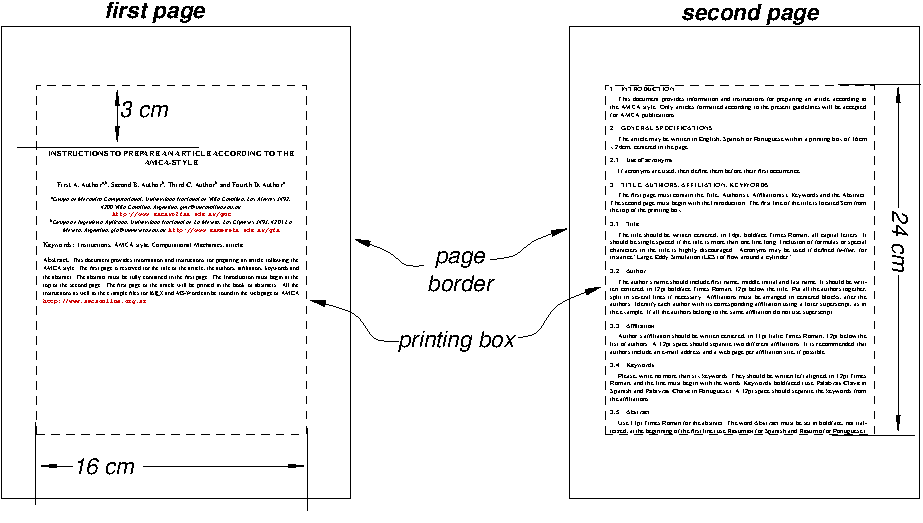
\includegraphics{firstpage}}
%\caption{Page layout}
%\label{fg:figure}
%\end{figure*}

%A 6pt space should separate the figure from the caption, and a
%12pt space should separate the upper part of the figure and the
%bottom of the caption from the surrounding text (see
%Fig.~\ref{fg:figure}).

%Figures should be referenced in the text. Color figures are welcomed.

%\section{EQUATIONS}

%A displayed equation is numbered, using Arabic numbers in parentheses.
%It should be  centered, leaving a 6pt space above and below to separate it from
%the surrounding text.

%The following example is a simple single line
%equation
%
%\begin{equation}
%Ax = b.
%\end{equation}

%The next example is a multi-line equation
%
%\begin{equation} \label{eq:simple}  
%\begin{aligned}
%Ax& = b,\\
%Ax& = c.
%\end{aligned}
%\end{equation}
%
%If possible, internal PDF links must be generated for references to
%equations. The recommended color for links to references in the text
%is blue (e.g., see Eq.~(\ref{eq:simple})).

%\section{TABLES}

%All tables should be numbered consecutively and captioned, the caption
%should be 10pt Times Roman, upper and lower case letters.

%A space of 6pt separates the table from the caption, and 12pt space
%separates the table from the surrounding text. For an example, see
%Table~\ref{tab:n50}. Tables should be referenced in the text.

%\begin{table}[htb]
%\centering
%\begin{tabular}{|c|c|c|c|}
%\hline  & 20x20 mesh & 50x50 mesh & 100x100 mesh\\
%\hline
%\hline
% 0 & 41.00 & 1.00 & 4.92\\
%\hline
% 1 & 40.86 & 1.02 & 4.88 \\
%\hline
%10 & 23.81 & 3.44 & 2.92 \\
%\hline
%50 & 5.62 & 64.20 & 1.08 \\
%\hline
%\end{tabular}
%\caption{Condition number for the Stekhlov operator. }
%\label{tab:n50}
%\end{table}

%\section{FORMAT OF REFERENCES}

%References should be quoted in the text using the \emph{author-style}
%(a.k.a. \emph{Harvard style}). References can be cited in
%\emph{parenthetical} form \citep{zienkiewicz91,idelsohn94,meyer82,meyer82b}, or
%in \emph{textual} form, e.g. see
%\citet{zienkiewicz91,idelsohn94,meyer82,meyer82b}.  References are grouped
%together and sorted alphabetically at the end of the article as shown
%in these instructions. Do not include references that are not cited in
%the article body. 

%If possible, internal PDF links must be generated for citations. The
%recommended color for links to references in the text is blue. The
%preferred color for links to external references, as web pages, 
%is red (e.g. \url{http://www.amcaonline.org.ar}).

\section{CONCLUSIONS}

In this paper the transmittance model of DVR is applied in the GPU to a 3D scalar field representing the bread crumb structure, to obtain realistic bread crumb images. This structure is generated using particle systems in which particles follow dynamical systems in a probabilistic way. A numerical simulation is employed to solve the resulting set of equations which represents the dynamical system. Results show high fidelity images in real time, suitable for application in several areas, such as serious games \citep{Susi2007} and photo-realistic rendering. This procedure does not present the drawbacks of other state of the art methods, such as capture processes or mesh generation.

The main disadvantage of the method is resolution, since close look-ups of the structure could lead to homogeneous areas due to hardware constraints, {\em i.e.}, arbitrary texture sizes are not allowed. This disadvantage is not exclusive of our method. A number of possible solutions will be employed to overcome this problem, such as setting different volume textures depending on the distance to the volume. 

As possible continuations of this work, DVR could be extended to handle other phenomena such as indirect illumination and sub surface scattering in order to enhance the images obtained. Also, partial differential equations will be employed to implement the baking process of bread \citep{Purlis2012}. Other porous materials such as cheeses will be investigated. Another interesting work will be to define primitives for crumb and crust modelling (shapes and intersections), enabling artists to define its shape.

%Template files in TeX, \LaTeX{} and MS-Word may be found at the
%AMCA web site: \url{http://www.amcaonline.org.ar}. 
%Remember: {\bf Do not number the pages.}
%
\bibliography{eniefbib}
\end{document}
% $Id: amcapaper.tex,v 1.23 2006/08/14 16:58:45 mstorti Exp $
